% Reproducible experiment; numerical macros are generated from C++ output.
% Generated by scripts/make_figures.py
\newcommand{\AttBest}{10628}
\newcommand{\AttInitial}{49454}
\newcommand{\AttTemperature}{2522.862044}
\newcommand{\AttProposals}{2\,188\,800}
\newcommand{\AttAccepted}{346\,966}
\newcommand{\AttFirstBest}{1\,076\,288}
\newcommand{\AttMean}{10687.70}
\newcommand{\AttMedian}{10673.00}
\newcommand{\AttStd}{54.55}
\newcommand{\AttWorst}{10840}
\newcommand{\AttHits}{3}
\newcommand{\AttMeanGap}{0.562}
\newcommand{\AttReduction}{78.51}
\newcommand{\AttMeanTime}{0.0726}

\section{经典实例实验：美国本土 48 州首府}
\subsection{数据来源、地图与距离定义}
选用 TSPLIB 的 \texttt{att48} 实例。官方文件说明为“48 capitals of the US
(Padberg/Rinaldi)”，含 48 个城市，类型为对称 TSP，边权类型为
\texttt{ATT}\cite{tsplib}。它对应美国本土相连 48 州的首府，不含阿拉斯加、
夏威夷及华盛顿特区。固定起点并去除反向重复后有 $47!/2$ 条不同回路，
适合在普通计算机上观察启发式搜索。

原始文件 \texttt{data/att48.tsp} 与参考路线 \texttt{data/att48.opt.tour}
均从海德堡大学 TSPLIB 官方站点获取。官方公布的最优费用为
$C^\star=10628$\cite{attbest}。参考路线仅用于独立验证，\textbf{不参与初始化、
搜索或停止判断}。本节在输入输出中使用 TSPLIB 的 $1,\ldots,48$ 编号，
C++ 内部仍使用从 0 开始的下标。

ATT 坐标不是经纬度；按 TSPLIB 定义，令
\begin{equation}
 r_{ij}=\sqrt{\frac{(x_i-x_j)^2+(y_i-y_j)^2}{10}},\quad
 t_{ij}=\left\lfloor r_{ij}+\frac12\right\rfloor,\quad
 d_{ij}=\begin{cases}t_{ij}+1,&t_{ij}<r_{ij},\\t_{ij},&t_{ij}\geq r_{ij}.\end{cases}
 \label{eq:att-distance}
\end{equation}
因此总费用是整数 ATT 单位，不能解释为公里或实际公路里程。
地理图采用 Natural Earth 的州界和首府位置\cite{naturalearth}；按照州名的
英文字母顺序，将本土 48 州的首府与实例编号对应。经纬度只用于地图展示，
所有优化及费用计算均使用原始坐标和\cref{eq:att-distance}。

\begin{figure}[htbp]
 \centering
 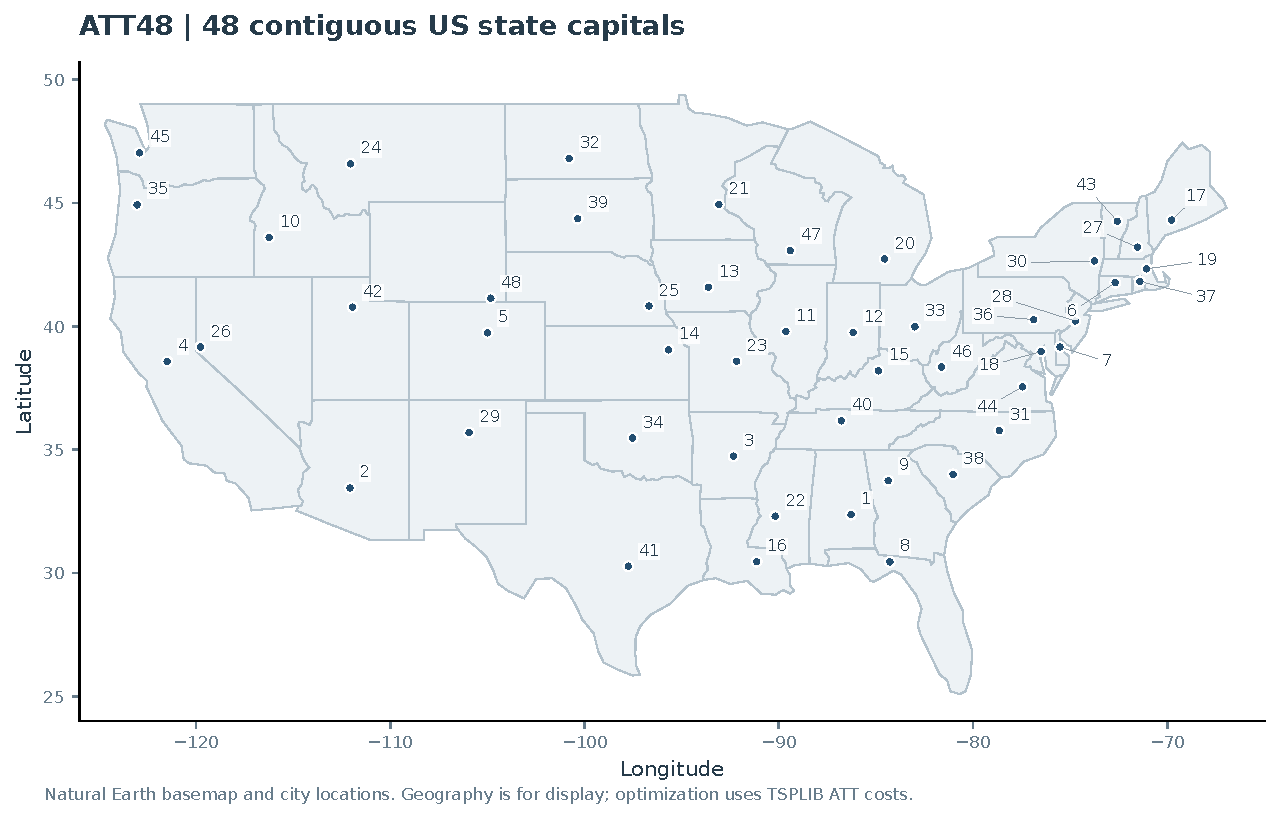
\includegraphics[width=.98\linewidth]{figures/att48_map.pdf}
 \caption{ATT48 对应的美国本土 48 州首府地理示意图。数字为 TSPLIB 节点编号；
 州界为概化底图。完整编号、州名、首府与经纬度见 \texttt{data/att48\_capitals.csv}。}
 \label{fig:att-map}
\end{figure}

\clearpage
\subsection{C++ 实现与每一步搜索的可视化}
\texttt{src/tsp.hpp} 实现数据解析、整数距离矩阵、初温采样和模拟退火；
\texttt{src/main.cpp} 处理用户选项并导出实验记录；
\texttt{src/visualizer.hpp} 使用 Windows 原生 GDI 窗口绘制路线。
求解器采用 C++17，不依赖第三方图形库；无界面求解也可在其他支持 C++17 的系统编译。
Python 仅用于实验后的绘图，不承担本节 TSP 求解。

算法沿用前文的随机初始排列、200 次初温试采样、2-opt 提案、Metropolis 接受准则、
几何降温与历史最好解保存。使用 64 位整数保存边权及路径费用，避免 ATT 费用累积误差。
核心循环中的更新和可视化调用如下（省略外围变量定义）：
\begin{lstlisting}[language=C++]
const auto [i, j] = rng.pair(n);
const Cost change = delta(route, p.distance, i, j);
const bool accept = change <= 0 ||
    rng.uniform() < std::exp(-double(change) / temperature);
++out.proposals;
if (accept) {
    std::reverse(route.begin()+i, route.begin()+j+1);
    current += change;
    ++out.accepted;
    if (current < out.best) {
        out.best = current;
        out.route = route;
        out.best_iteration = out.proposals;
    }
}
if (observer && !observer({out.proposals, out.levels+1,
        temperature, current, out.best, accept, route, out.route}))
    observer = {};
\end{lstlisting}

\textbf{一步的定义。}一次 2-opt 候选提案为一步，包含接受和拒绝。
每一步接受判断结束后，界面同步重绘\emph{当前路线}、当前费用、历史最好费用、温度和
提案计数；被拒绝时同一路线仍会刷新。初始化也绘制一次。
程序在该帧绘制完成之后才生成下一次候选，不按温度层抽帧，也不只显示改善。
最终搜索结束时显示历史最好路线。

\textbf{运行中的控制。}空格暂停或继续；\texttt{N} 在暂停状态下前进一步；
加减号调整帧间等待；\texttt{Esc}、\texttt{V} 或窗口关闭按钮立即关闭可视化。
关闭时仅移除绘图回调，原有随机数流和退火状态继续使用，最终结果照常写盘。
界面暂停时仍处理关闭事件；可视化不消耗求解器随机数，故开关显示不改变搜索结果。

\begin{keypoint}{展示速度与计算速度}
默认每帧至少等待 16 毫秒，完整的 2\,188\,800 次提案仅帧等待就约需 9.7 小时。
这属于逐步展示开销。需要快速获得答案时应关闭显示；演示时可缩减提案预算。
无界面运行的计时不能与启用显示的计时直接比较。
\end{keypoint}

\clearpage
\subsection{实验设置、结果与地图上的闭环}
实验采用 Windows、GCC 15.2.0、C++17 和 \texttt{-O2}，关闭可视化计时。
每个温度提出 $L=4800$ 次候选，取 $\alpha=0.98$、$T_{\min}/T_0=10^{-4}$、
$K_{\max}=2000$，实际执行 456 层。使用预先确定的连续随机种子 42 至 61，
共进行 20 次独立运行。每次重新生成随机初始路线和初温，不加入局部精修或参考最优路线。

种子 42 的初温为 $T_0=\AttTemperature$；总计提出 \AttProposals{} 次候选，
接受 \AttAccepted{} 次，在第 \AttFirstBest{} 次提案首次找到费用 10628 的路线。
初始费用为 \AttInitial，最终减少了 \AttReduction\%。它与公开最优费用一致，
因此这次输出达到了该实例的已知全局最优值；这种结论依赖外部基准，
不能推广为模拟退火对其他种子或实例的最优性保证。

\begin{figure}[htbp]
 \centering
 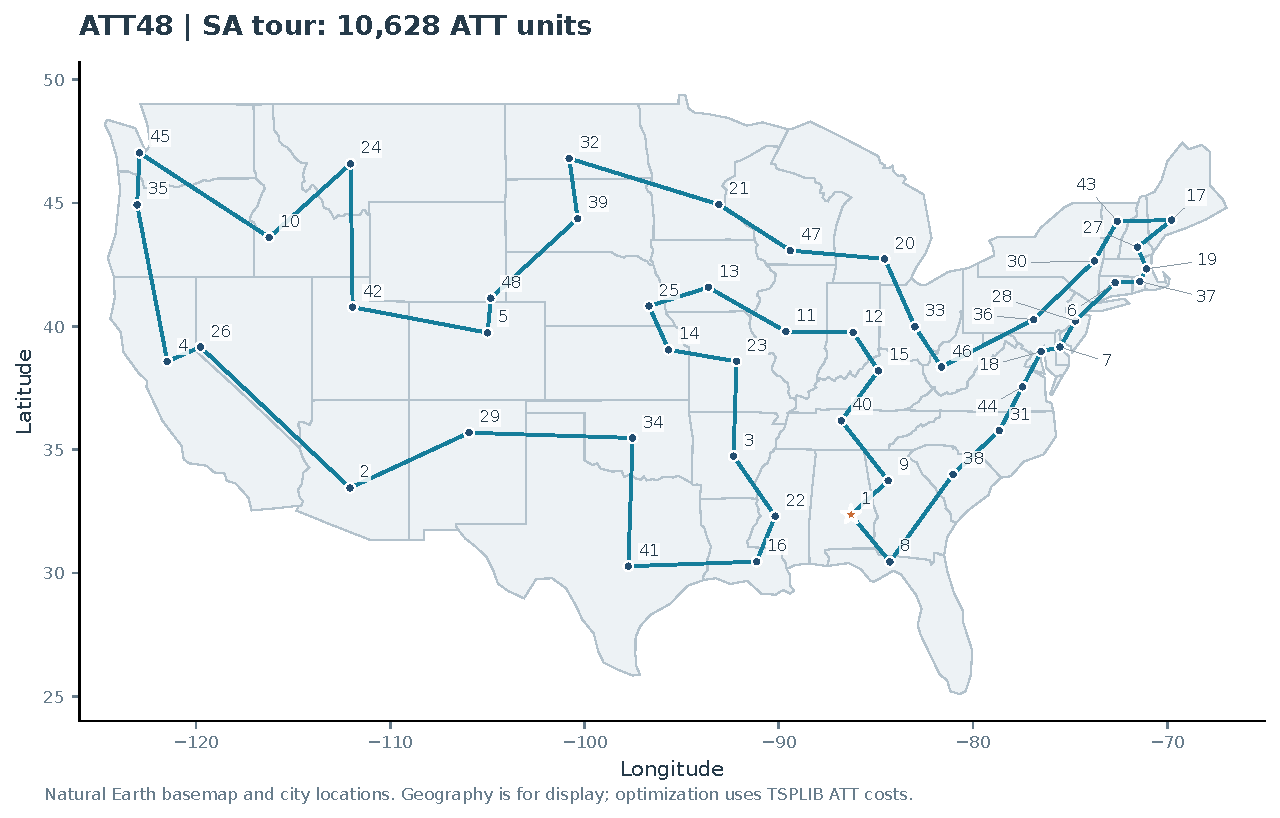
\includegraphics[width=.98\linewidth]{figures/att48_solution.pdf}
 \caption{种子 42 得到的最好闭环在地理地图上的展示，费用为 10628 ATT 单位，
 与官方最优值相同。橙色星形为节点 1（Alabama 州 Montgomery 首府），
 连线表示访问关系，并非实际道路。返回节点 1 的边已计入费用。}
 \label{fig:att-solution}
\end{figure}

完整访问顺序如下；按行连接，最后一个 1 表示返回起点：
\lstinputlisting[basicstyle=\ttfamily\small]{results/att48/route.txt}

\clearpage
\subsection{收敛过程与重复实验}
\cref{fig:att-convergence}展示种子 42 的费用变化。浅色曲线为每个温度层结束时的当前费用，
蓝色阶梯线为同一时刻的历史最好费用，虚线为公开最优值。
前期高温允许接受变差，当前费用存在明显起伏；随着温度降低，当前路线逐渐接近
历史最好路线。后者按定义单调不增。记录文件保存初始状态及全部 456 个温度层的末状态，
因此图中曲线是 457 个采样点；\textbf{这与实时窗口逐提案重绘的频率不同}。
首次最优解的提案编号由求解器单独记录，未由曲线采样位置估计。

\begin{figure}[htbp]
 \centering
 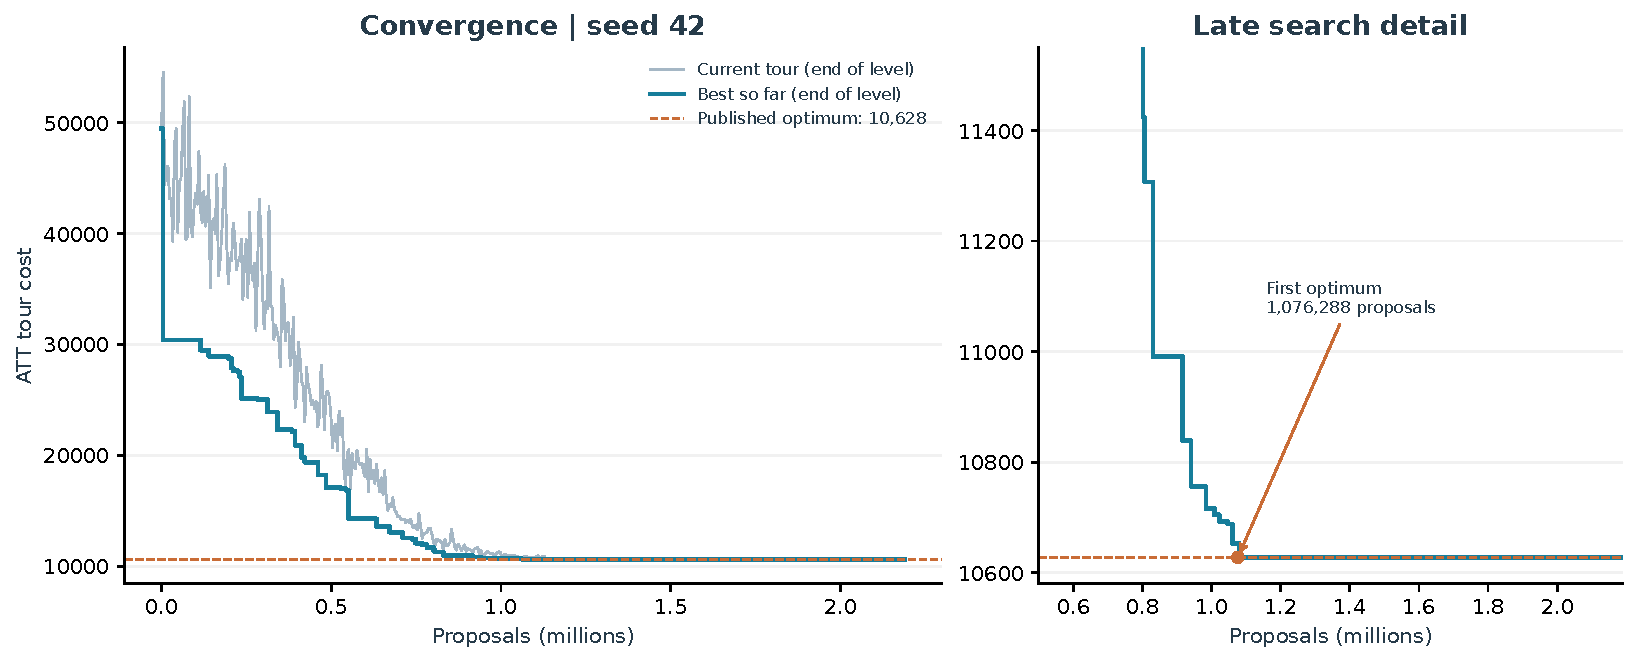
\includegraphics[width=\linewidth]{figures/att48_convergence.pdf}
 \caption{ATT48 模拟退火的收敛曲线及后期放大图。横轴为提案次数（百万），
 纵轴为闭环总费用；拒绝的候选也计入提案数。}
 \label{fig:att-convergence}
\end{figure}

\begin{table}[htbp]
 \centering\small
 \caption{20 次独立运行的实测结果；费用均为 ATT 单位，标准差采用样本标准差}
 \label{tab:att-results}
 \begin{tabularx}{.95\linewidth}{@{}XrXr@{}}
 \toprule
 指标 & 数值 & 指标 & 数值\\
 \midrule
 最好费用 & \AttBest & 最差费用 & \AttWorst\\
 平均费用 & \AttMean & 中位数 & \AttMedian\\
 样本标准差 & \AttStd & 达到最优值 & \AttHits/20\\
 平均相对差距 & \AttMeanGap\% & 平均单次求解时间 & \AttMeanTime{} s\\
 \bottomrule
 \end{tabularx}
\end{table}
相对差距定义为 $100(C-10628)/10628$。求解计时从初始排列生成前开始，
覆盖初温标定、全部搜索和内存中的记录，不包括数据读取、文件输出、绘图与编译。
短时间测量会受本机调度影响，不能直接视为其他计算机的运行时间。
20 次运行中只有 3 次达到最优值，说明即使在同一实例和预算下，随机种子也会影响结果。

\begin{figure}[!htbp]
 \centering
 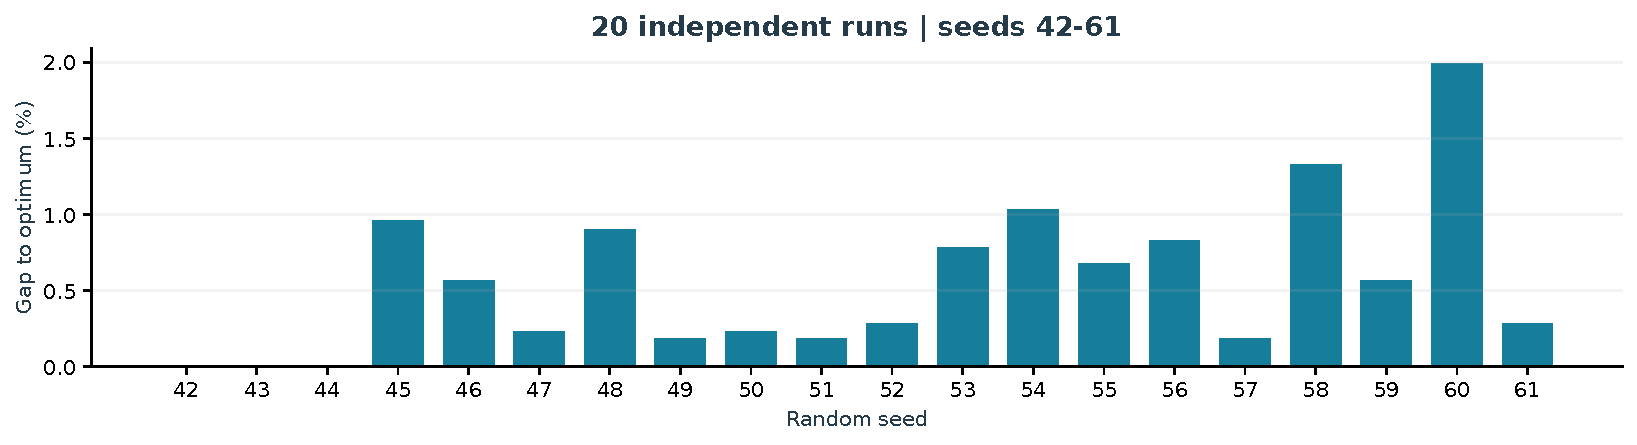
\includegraphics[width=.97\linewidth]{figures/att48_runs.pdf}
 \caption{连续种子 42--61 的最终费用相对于公开最优值的差距。零高度对应达到最优值。}
 \label{fig:att-runs}
\end{figure}

\clearpage
\subsection{复现命令与独立验证}
在项目根目录用 MinGW-w64 编译并运行。程序不带显示选项时，会在终端询问
\texttt{Visualize every proposal? [y/N]}；也可以通过选项直接决定：
\begin{lstlisting}[language=bash]
g++ -std=c++17 -O2 -static src/main.cpp -o build/tsp_sa.exe -lgdi32 -luser32
build/tsp_sa.exe --visual
build/tsp_sa.exe --no-visual --runs 20 --output results/att48
python scripts/verify_results.py
python scripts/make_figures.py
xelatex -output-directory=output/pdf tsp_simulated_annealing.tex
xelatex -output-directory=output/pdf tsp_simulated_annealing.tex
\end{lstlisting}
也可执行 \texttt{build.ps1} 自动创建编译目录。完整数据、图件和本节使用的结果已随项目保存，
无需重新联网即可编译文档；需要重绘时安装 \texttt{requirements-figures.txt} 中的依赖。
每个种子独立保存 \texttt{result.json}、\texttt{history.csv} 和 \texttt{best.tour}；
总目录的 \texttt{runs.csv} 汇总所有运行，\texttt{result.json} 保存这批运行中的最好结果。
本节数值宏与图件均由同一份结果文件自动生成。

\begin{figure}[htbp]
 \centering
 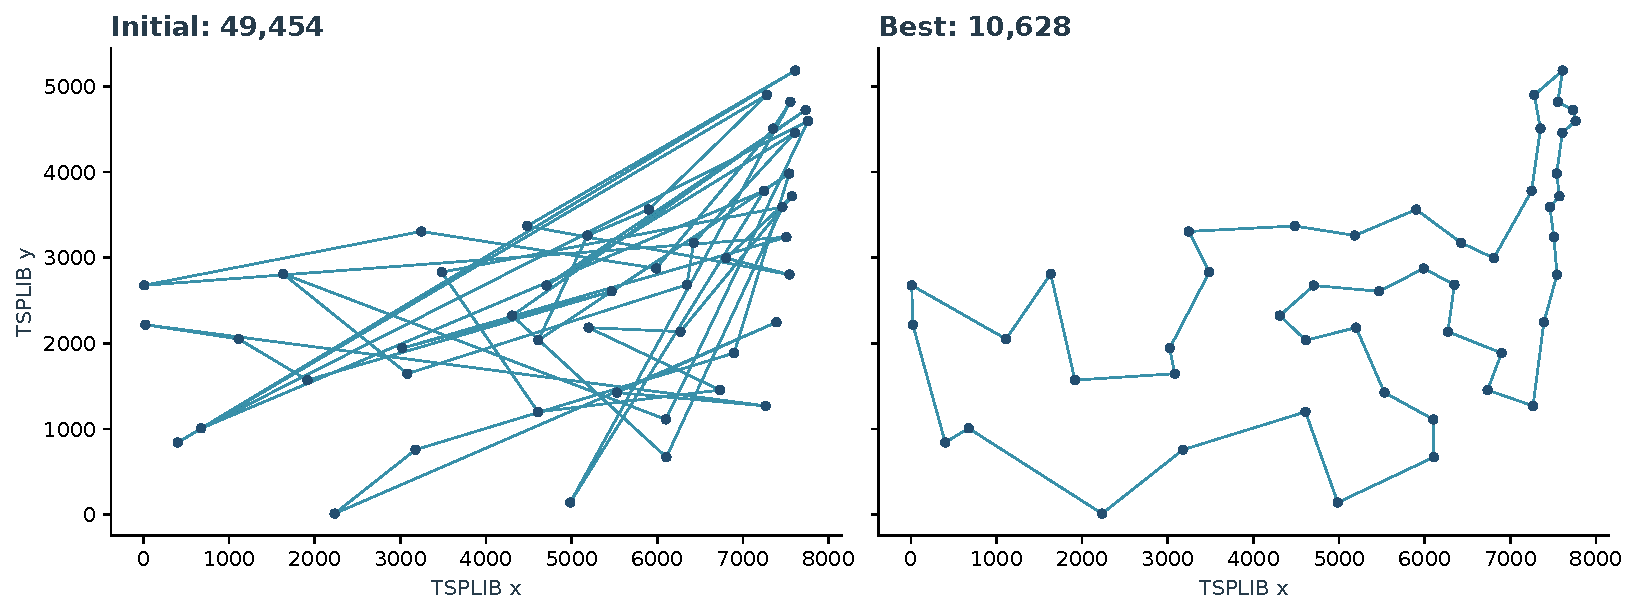
\includegraphics[width=\linewidth]{figures/att48_coordinate_tours.pdf}
 \caption{原始 TSPLIB 坐标系中的随机初始路线与求得的最好路线。
 本图直接使用求解坐标，不使用地理地图上的经纬度；两幅图采用相同尺度。}
 \label{fig:att-coordinates}
\end{figure}

\textbf{验证覆盖。}C++ 测试独立读取官方最优路线，按 ATT 规则重算得到 10628；
对 10 个随机排列中的全部位置对进行 10\,810 次四边增量与完整重算核对，包含返回起点边。
另检查小实例精确值、零距离、参数校验、固定种子复现、每次提案回调以及拒绝提案的刷新。
Windows 集成测试在真实窗口中验证暂停、单步及暂停状态下的三种关闭方式，
确认移除显示后仍完成全部提案，且路线和接受次数与无显示运行相同。
Python 校验脚本对全部 20 次实验逐一重算费用、检查完整排列、预算和收敛记录的单调性。
